\section[pbdMPI]{Introduction to pbdMPI}

\hidenum
\begin{frame}[noframenumbering]
\frametitle{Contents}
 \tableofcontents[currentsection,hideothersubsections,sectionstyle=show/hide]
\end{frame}
\shownum

\subsection{Managing a Communicator}

\begin{frame}
  \begin{block}{Message Passing Interface (MPI)}\pause
    \begin{itemize}
      \item \textit{MPI}: Standard for managing communications (data and instructions) between different nodes/computers.
      \item \textit{Implementations}:  OpenMPI, MPICH2, Cray MPT, \dots
      \item Enables parallelism on distributed machines.
      \item \textit{Communicator}: manages communications between processors.
    \end{itemize}
  \end{block}
\end{frame}


\begin{frame}
  \begin{block}{MPI Operations (1 of 2)}\pause
    \begin{itemize}
      \item \textbf{Managing a Communicator}:  Create and destroy communicators.\\
      \code{init()} --- initialize communicator\\
      \code{finalize()} --- shut down communicator(s)
      \\[.4cm]
      %
      \item \textbf{Rank query}: determine the processor's position in the communicator.\\
      \code{comm.rank()} --- ``who am I?''\\
      \code{comm.size()} --- ``how many of us are there?''\\[.4cm]
      \item \textbf{Printing}:  Printing output from various ranks.\\
      \code{comm.print(x)}\\
      \code{comm.cat(x)}\\
      \textbf{WARNING}: only use these functions on \emph{results}, never on yet-to-be-computed things.\\
    \end{itemize}
  \end{block}
\end{frame}


\begin{frame}[fragile]
  \begin{exampleblock}{Quick Example 1}
  \centering
\begin{lstlisting}[title=Rank Query: 1\_rank.r]
library(pbdMPI, quiet = TRUE)
init()

my.rank <- comm.rank()
comm.print(my.rank, all.rank=TRUE)

finalize()
\end{lstlisting}
  \begin{columns}[t,onlytextwidth]
    \begin{column}{0.62\textwidth}
\begin{lstlisting}[backgroundcolor=\color{white},keywordstyle=\color{black},title=Execute this script via:]
mpirun -np 2 Rscript 1_rank.r
\end{lstlisting}    
    \end{column}
    \hfill
    \begin{column}{0.35\textwidth}
\begin{lstlisting}[title=Sample Output:]
COMM.RANK = 0
[1] 0
COMM.RANK = 1
[1] 1
\end{lstlisting}
    \end{column}
​  \end{columns}
  \end{exampleblock}
\end{frame}



\begin{frame}[fragile]
  \begin{exampleblock}{Quick Example 2}
\begin{lstlisting}[title=Hello World: 2\_hello.r]
library(pbdMPI, quiet=TRUE)
init()

comm.print("Hello, world")

comm.print("Hello again", all.rank=TRUE, quiet=TRUE)

finalize()
\end{lstlisting}
  \begin{columns}[t,onlytextwidth]
    \begin{column}{0.58\textwidth}
\begin{lstlisting}[backgroundcolor=\color{white},keywordstyle=\color{black},title=Execute this script via:]
mpirun -np 2 Rscript 2_hello.r
\end{lstlisting}    
    \end{column}
    \hfill
    \begin{column}{0.4\textwidth}
\begin{lstlisting}[title=Sample Output:]
COMM.RANK = 0
[1] "Hello, world"
[1] "Hello again"
[1] "Hello again"
\end{lstlisting}
    \end{column}
​  \end{columns}
  \end{exampleblock}
\end{frame}



\subsection{Reduce, Gather, Broadcast, and Barrier}


\begin{frame}
  \begin{block}{MPI Operations}
    \begin{enumerate}
      \item Reduce
      \item Gather
      \item Broadcast
      \item Barrier
    \end{enumerate}
  \end{block}
\end{frame}

\begin{frame}
  \begin{block}{Reductions --- Combine results into single result}
    \begin{center}
      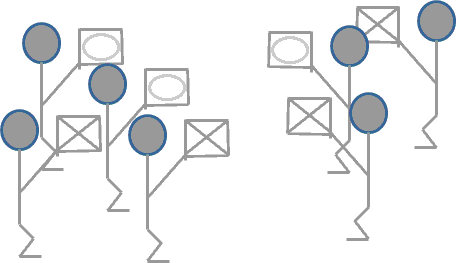
\includegraphics[scale=.6]{pics/mpi_reduce}
    \end{center}
  \end{block}
\end{frame}


\begin{frame}
  \begin{block}{Gather --- Many-to-one}
    \begin{center}
      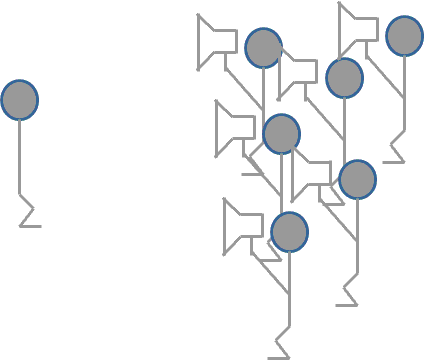
\includegraphics[scale=.6]{pics/mpi_gather}
    \end{center}
  \end{block}
\end{frame}


\begin{frame}
  \begin{block}{Broadcast --- One-to-many}
    \begin{center}
      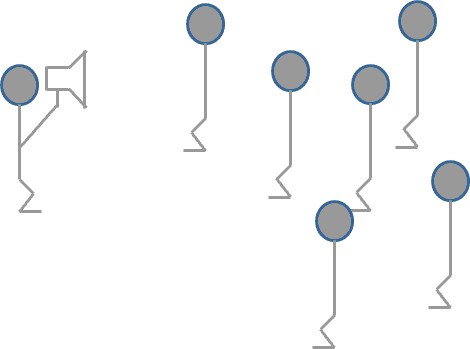
\includegraphics[scale=.6]{pics/mpi_bcast}
    \end{center}
  \end{block}
\end{frame}


\begin{frame}
  \begin{block}{Barrier --- Synchronization}
    \begin{center}
      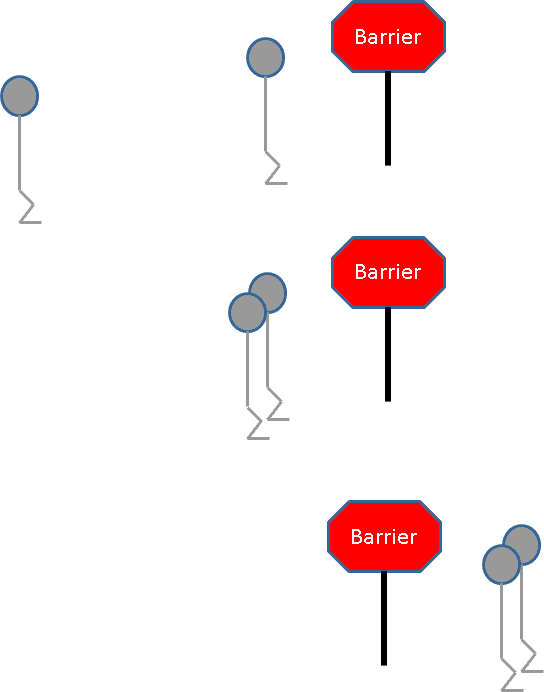
\includegraphics[scale=.38]{pics/mpi_barrier}
    \end{center}
  \end{block}
\end{frame}



\begin{frame}[shrink]
  \begin{block}{MPI Operations (2 of 2)}\pause
    \begin{itemize}
      \item \textbf{Reduction}:  each processor has a number \code{x}; add all of them up, find the largest/smallest, \dots .\\
      \code{reduce(x, op='sum')} --- reduce to one\\
      \code{allreduce(x, op='sum')} --- reduce to all\\[.4cm]
      %
      \item \textbf{Gather}: each processor has a number; create a new object on some processor containing all of those numbers.\\
      \code{gather(x)} --- gather to one\\
      \code{allgather(x)} --- gather to all\\[.4cm]
      %
      \item \textbf{Broadcast}: one processor has a number \code{x} that every other processor should also have.\\
      \code{bcast(x)}
      \\[.4cm]
      \item \textbf{Barrier}: ``computation wall''; no processor can proceed until \emph{all} processors can proceed.\\
\code{barrier()}
    \end{itemize}
  \end{block}
\end{frame}




\begin{frame}[fragile,shrink]
  \begin{exampleblock}{Quick Example 3}
\begin{lstlisting}[title=Reduce and Gather: 3\_gt.r]
library(pbdMPI, quiet = TRUE)
init()

comm.set.seed(diff=TRUE)

n <- sample(1:10, size=1)

gt <- gather(n)
comm.print(unlist(gt))

sm <- allreduce(n, op='sum')
comm.print(sm, all.rank=T)

finalize()
\end{lstlisting}
  \begin{columns}[t,onlytextwidth]
    \begin{column}{0.58\textwidth}
\begin{lstlisting}[backgroundcolor=\color{white},keywordstyle=\color{black},title=Execute this script via:]
mpirun -np 2 Rscript 3_gt.r
\end{lstlisting}    
    \end{column}
    \hfill
    \begin{column}{0.4\textwidth}
\begin{lstlisting}[title=Sample Output:]
COMM.RANK = 0
[1] 2 8
COMM.RANK = 0
[1] 10
COMM.RANK = 1
[1] 10
\end{lstlisting}
    \end{column}
​  \end{columns}
  \end{exampleblock}
\end{frame}


\begin{frame}[fragile,shrink]
  \begin{exampleblock}{Quick Example 4}
\begin{lstlisting}[title=Broadcast: 4\_bcast.r]
library(pbdMPI, quiet=T)
init()

if (comm.rank()==0){
  x <- matrix(1:4, nrow=2)
} else {
  x <- NULL
}

y <- bcast(x, rank.source=0)

comm.print(y, rank=1)

finalize()
\end{lstlisting}
  \begin{columns}[t,onlytextwidth]
    \begin{column}{0.58\textwidth}
\begin{lstlisting}[backgroundcolor=\color{white},keywordstyle=\color{black},title=Execute this script via:]
mpirun -np 2 Rscript 4_bcast.r
\end{lstlisting}
\end{column}
    \hfill
    \begin{column}{0.4\textwidth}
\begin{lstlisting}[title=Sample Output:]
COMM.RANK = 1
     [,1] [,2]
[1,]    1    3
[2,]    2    4
\end{lstlisting}
    \end{column}
​  \end{columns}
  \end{exampleblock}
\end{frame}







\subsection{Other }


\begin{frame}
  \begin{block}{MPI Package Controls}
The \code{.SPMD.CT} object allows for setting different package options with \pkg{pbdMPI}.  See the entry \emph{SPMD Control} of the \pkg{pbdMPI} manual for information about the \code{.SPMD.CT} object:
\begin{center}
{ \small
\url{http://cran.r-project.org/web/packages/pbdMPI/pbdMPI.pdf}
}
\end{center}
  \end{block}
\end{frame}

\begin{frame}[fragile,shrink]
  \begin{exampleblock}{Quick Example 5}
\begin{lstlisting}[title=Barrier: 5\_barrier.r]
library(pbdMPI, quiet = TRUE)
init()

.SPMD.CT$msg.barrier <- TRUE
.SPMD.CT$print.quiet <- TRUE

for (rank in 1:comm.size()-1){
  if (comm.rank() == rank){
    cat(paste("Hello", rank+1, "of", comm.size(), "\n"))
  }
  barrier()
}

comm.cat("\n")

comm.cat(paste("Hello", comm.rank()+1, "of", comm.size(), "\n"), all.rank=TRUE)

finalize()
\end{lstlisting}
  \begin{columns}[t,onlytextwidth]
    \begin{column}{0.58\textwidth}
\begin{lstlisting}[backgroundcolor=\color{white},keywordstyle=\color{black},title=Execute this script via:]
mpirun -np 2 Rscript 5_barrier.r
\end{lstlisting}
    \end{column}
    \hfill
    \begin{column}{0.4\textwidth}
\begin{lstlisting}[title=Sample Output:]
Hello 1 of 2 
Hello 2 of 2 
\end{lstlisting}
    \end{column}
​  \end{columns}
  \end{exampleblock}
\end{frame}


\begin{frame}
  \begin{block}{Random Seeds}\pause
  \pkg{pbdMPI} offers a simple interface for managing random seeds:
    \begin{itemize}
      \item \code{comm.set.seed(diff=TRUE)} --- Independent streams via the \pkg{rlecuyer} package.
      \item \code{comm.set.seed(seed=1234, diff=FALSE)} --- All processors use the same seed \code{seed=1234}
      \item \code{comm.set.seed(diff=FALSE)} --- All processors use the same seed, determined by processor 0 (using the system clock and PID of processor 0).
    \end{itemize}
  \end{block}
\end{frame}



\begin{frame}[fragile,shrink]
  \begin{exampleblock}{Quick Example 6}
\begin{lstlisting}[title=Timing: 6\_timer.r]
library(pbdMPI, quiet=TRUE)
init()

comm.set.seed(diff=T)

test <- function(timed)
{
  ltime <- system.time(timed)[3]
  
  mintime <- allreduce(ltime, op='min')
  maxtime <- allreduce(ltime, op='max')
  meantime <- allreduce(ltime, op='sum')/comm.size()

  return(data.frame(min=mintime, mean=meantime, max=maxtime))
}

times <- test(rnorm(1e6)) # ~7.6MiB of data
comm.print(times)

finalize()
\end{lstlisting}
  \begin{columns}[t,onlytextwidth]
    \begin{column}{0.58\textwidth}
\begin{lstlisting}[backgroundcolor=\color{white},keywordstyle=\color{black},title=Execute this script via:]
mpirun -np 2 Rscript 6_timer.r
\end{lstlisting}
\end{column}
    \hfill
    \begin{column}{0.35\textwidth}
\begin{lstlisting}[title=Sample Output:]
   min  mean   max
1 0.17 0.173 0.176
\end{lstlisting}
\end{column}
\end{columns}
  \end{exampleblock}
\end{frame}



\begin{frame}
  \begin{block}{Other Helper Tools}\pause
  \pkg{pbdMPI} Also contains useful tools for Manager/Worker and task parallelism codes:
    \begin{itemize}
      \item \textbf{Task Subsetting}: Distributing a list of jobs/tasks\\ 
      \code{get.jid(n)}
      %
      \item \textbf{*ply}:  Functions in the *ply family.\\
      \code{pbdApply(X, MARGIN, FUN, \dots)} --- analogue of \code{apply()}\\
      \code{pbdLapply(X, FUN, \dots)} --- analogue of \code{lapply()}\\
      \code{pbdSapply(X, FUN, \dots)} --- analogue of \code{sapply()}\\
    \end{itemize}
  \end{block}
\end{frame}






\begin{frame}[fragile]
  \begin{block}{Quick Comments for Using pbdMPI}\pause
    \begin{enumerate}
      \item Start by loading the package:
\vspace{-.4cm}
\begin{lstlisting}
library(pbdMPI, quiet = TRUE)
\end{lstlisting}
      \item Always initialize before starting and finalize when finished:
\vspace{-.4cm}
\begin{lstlisting}
init()

# ...

finalize()
\end{lstlisting}
\end{enumerate}
\end{block}
\end{frame}